\subsection{Comparison between different correctors used (CPU time and iterations)}
\label{subsec:comparison_between_different_correctors_used}

Here follows a graphical comparison of the CPU time and the number of iterations for the different corrector methods used.

Notice that in the legend of the graphs, the following abbreviations are used:

\begin{itemize}
    \item \textbf{NR}: Newton-Raphson method
    \item \textbf{mNR}: modified Newton-Raphson method
\end{itemize}

\begin{table}[H]
    \centering
    \begin{tabular}{|c|c|c|}
        \hline
        \textbf{Parameter} & \textbf{Value} & \textbf{Unit} \\ \hline
        Number of steps    & $1$            & ~             \\ \hline
        $\Delta P_x$       & $5*10^{5}$     & N             \\ \hline
        $\Delta P_y$       & $5*10^{5}$     & N             \\ \hline
        Tolerance          & $10^{-7}$      & N             \\ \hline
    \end{tabular}
    \caption{Parameters used for the comparison}
    \label{tab:parameters_for_CPU_time_and_iterations_comparison}
\end{table}

\begin{figure}[H]
    \centering
    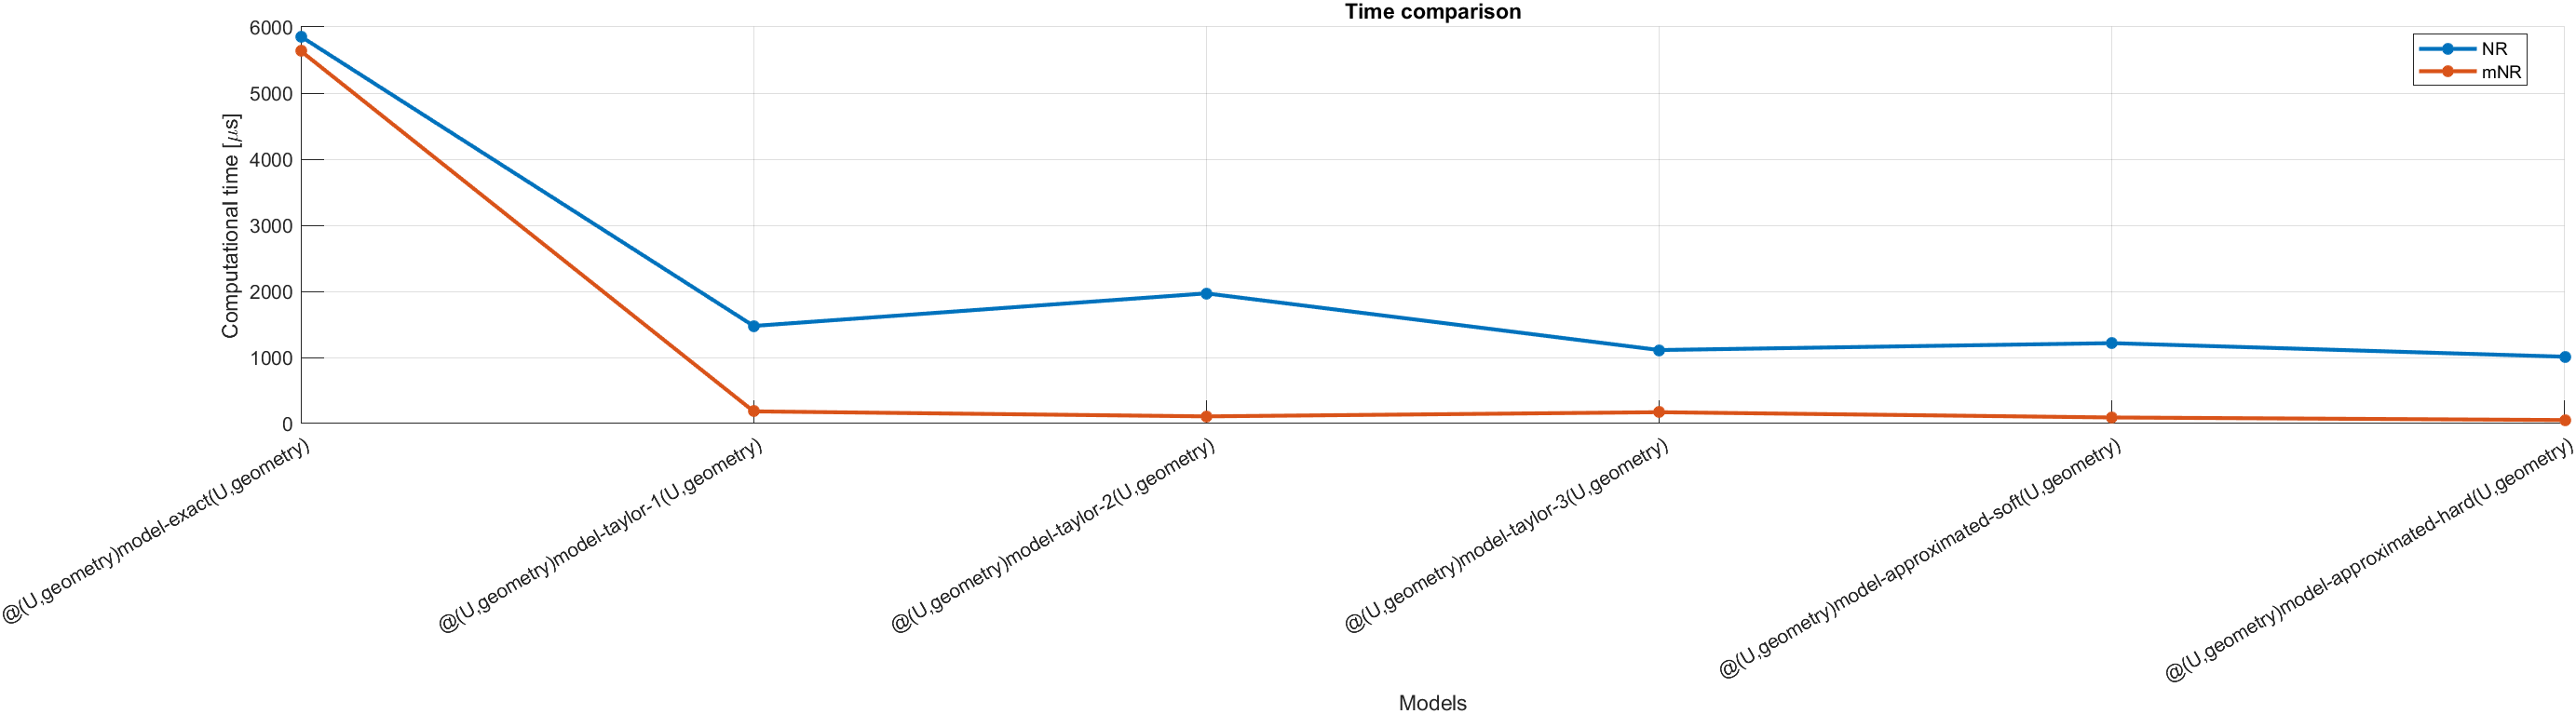
\includegraphics[width=.9\textwidth]{img/CPU_time_comparison}
    \caption{Comparison of CPU time for different correctors used.}
    \label{fig:CPU_time_comparison}
\end{figure}

\begin{figure}[H]
    \centering
    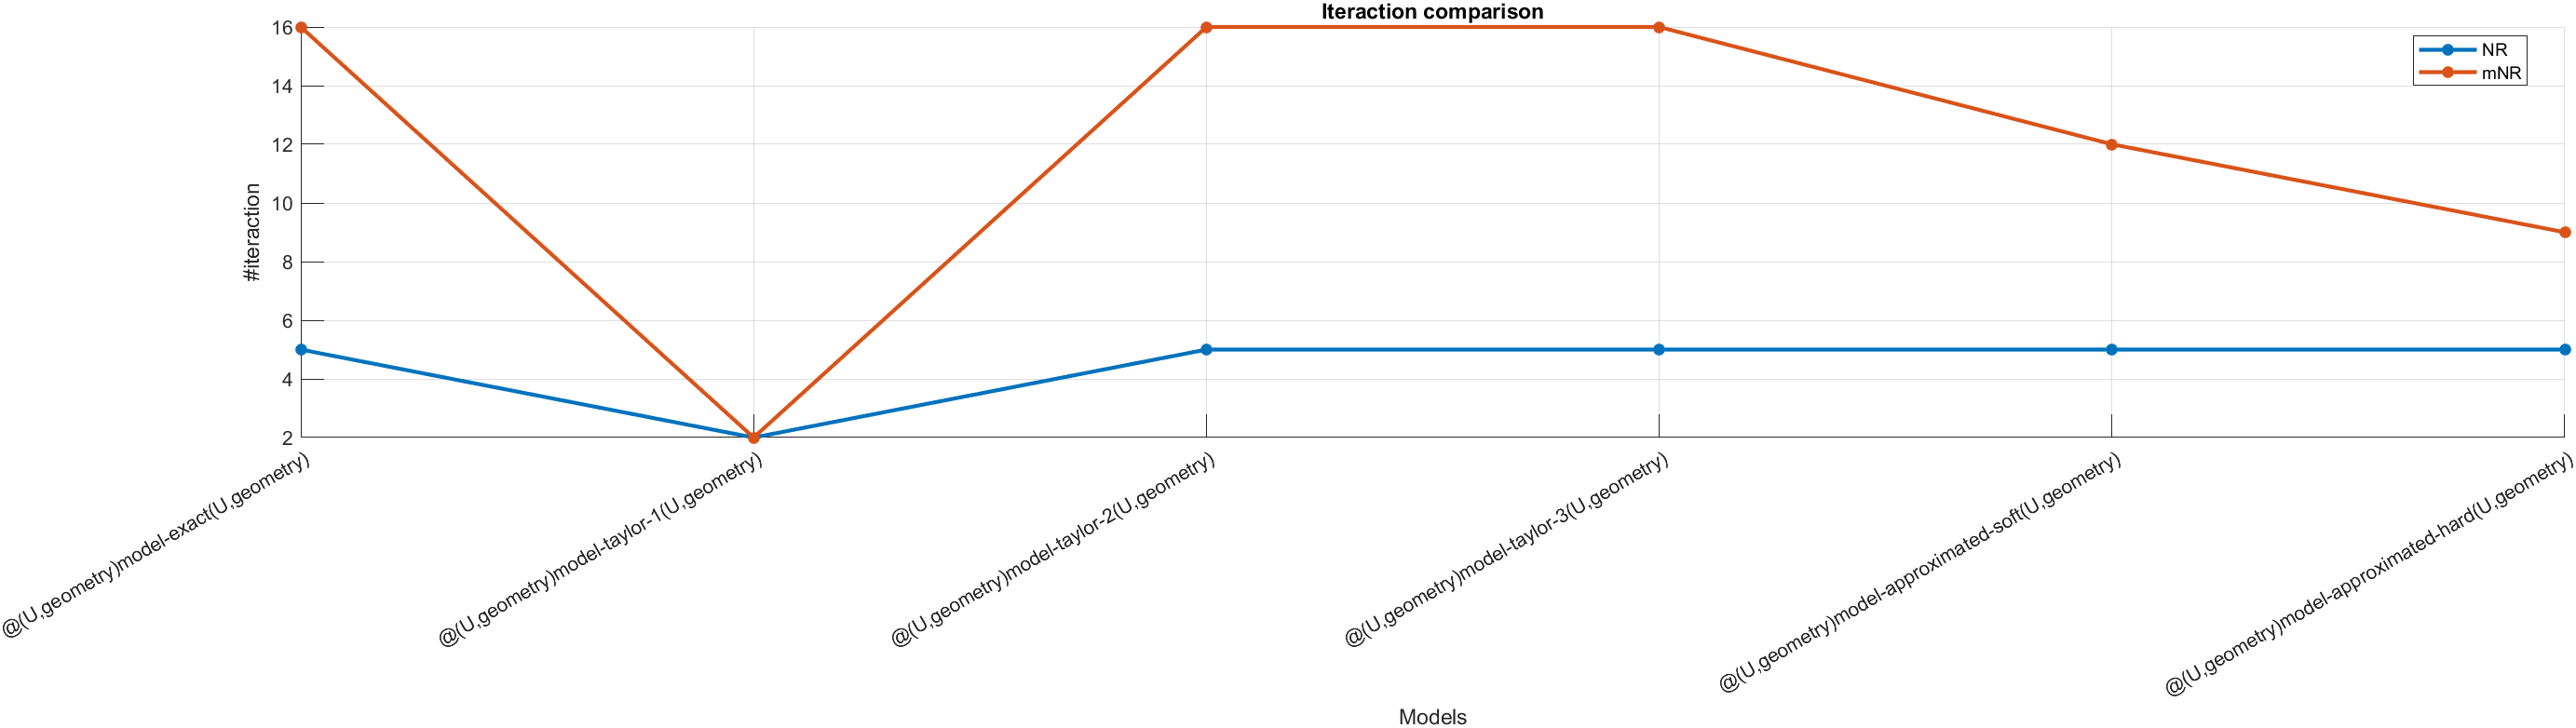
\includegraphics[width=.9\textwidth]{img/iterations_comparison}
    \caption{Comparison of number of iterations for different correctors used.}
    \label{fig:iterations_comparison}
\end{figure}

From the graph in Figure \ref{fig:CPU_time_comparison} we can see that the CPU time for the modified Newton-Raphson method is the lower then the one for the Newton-Raphson method.
Instead, in Figure \ref{fig:iterations_comparison} we can see that the number of iterations for the modified Newton-Raphson method is higher than the one for the Newton-Raphson method.

These results align with the theoretical expectations.
In the Newton-Raphson method, the computation of the inverse of $[K_{t,n}]$ at each iteration contributes to increased CPU time and enhanced precision in each step, corresponding to a lower iteration number.
On the other hand, in the modified Newton-Raphson method, the inverse of $[K_{t,n}]$ is computed only in the initial iteration, leading to reduced CPU time and precision per step, causing a higher iteration number.